
\documentclass[12pt,a4paper, oneside]{extreport}

%%%%%%%%%% Математика %%%%%%%%%%
\usepackage{amsmath,amsfonts,amssymb,amsthm,mathtools}
% Показывать номера только у тех формул, на которые есть \eqref{} в тексте.
%\mathtoolsset{showonlyrefs=true}
%\usepackage{leqno} % Нумерация формул слева
%\usepackage{tipa} %Для формулки из логитов


\usepackage{hyphenat}

%%%%%%%%%% Шрифты %%%%%%%%
\usepackage[english, russian]{babel} % выбор языка для документа
\usepackage[utf8]{inputenc} % задание utf8 кодировки исходного tex файла
\usepackage[X2,T2A]{fontenc}        % кодировка
%
\usepackage{fontspec}         % пакет для подгрузки шрифтов
\setmainfont{Times New Roman}       % задаёт основной шрифт документа

\usepackage{unicode-math}      % пакет для установки математического шрифта
%\setmathfont{Asana-Math.otf}    % шрифт для математики

% Конкретный символ из конкретного шрифта
% \setmathfont[range=\int]{Neo Euler}


%%%%%%%%%% Работа с картинками %%%%%%%%%
\usepackage{graphicx}                  % Для вставки рисунков
\usepackage{graphics}
\graphicspath{{images/}{pictures/}}    % можно указать папки с картинками
\usepackage{wrapfig}                   % Обтекание рисунков и таблиц текстом


%%%%%%%%%% Работа с таблицами %%%%%%%%%%
\usepackage{tabularx}            % новые типы колонок
\usepackage{tabulary}            % и ещё новые типы колонок
\usepackage{array,delarray}      % Дополнительная работа с таблицами
\usepackage{longtable}           % Длинные таблицы
\usepackage{multirow}            % Слияние строк в таблице
\usepackage{float}               % возможность позиционировать объекты в нужном месте

\usepackage{booktabs}            % таблицы как в книгах

% Заповеди из документации к booktabs:
% 1. Будь проще! Глазам должно быть комфортно
% 2. Не используйте вертикальные линни
% 3. Не используйте двойные линии. Как правило, достаточно трёх горизонтальных линий
% 4. Единицы измерения - в шапку таблицы
% 5. Не сокращайте .1 вместо 0.1
% 6. Повторяющееся значение повторяйте, а не говорите "то же"
% 7. Есть сомнения? Выравнивай по левому краю!

%  вычисляемые колонки по tabularx
\newcolumntype{C}{>{\centering\arraybackslash}X}
\newcolumntype{L}{>{\raggedright\arraybackslash}X}
\newcolumntype{Y}{>{\arraybackslash}X}
\newcolumntype{Z}{>{\centering\arraybackslash}X}


%%%%%%%%%% Графика и рисование %%%%%%%%%%
\usepackage{tikz, pgfplots}      % язык для рисования графики из latex'a

%%%%%%%%%% Гиперссылки %%%%%%%%%%
\usepackage{xcolor}              % разные цвета

\usepackage{hyperref}
\hypersetup{
	unicode=true,           % позволяет использовать юникодные символы
	colorlinks=true,       	% true - цветные ссылки, false - ссылки в рамках
	urlcolor =blue,         % цвет ссылки на url
	linkcolor=black,        % внутренние ссылки
	citecolor=black,        % на библиографию
	breaklinks              % если ссылка не умещается в одну строку, разбивать ли ее на две части?
}


%%%%%%%%%% Другие приятные пакеты %%%%%%%%%
\usepackage{multicol}       % несколько колонок
\usepackage{verbatim}       % для многострочных комментариев
\usepackage{cmap} % для кодировки шрифтов в pdf

\usepackage{enumitem} % дополнительные плюшки для списков
%  например \begin{enumerate}[resume] позволяет продолжить нумерацию в новом списке

\usepackage{todonotes} % для вставки в документ заметок о том, что  осталось сделать
% \todo{Здесь надо коэффициенты исправить}
% \missingfigure{Здесь будет Последний день Помпеи}
% \listoftodos --- печатает все поставленные \todo'шки



%%%%%%%%%%%%%% ГОСТОВСКИЕ ПРИБАМБАСЫ %%%%%%%%%%%%%%%

%%% размер листа бумаги
\usepackage[paper=a4paper,top=15mm, bottom=15mm,left=35mm,right=10mm,includehead]{geometry}


\usepackage{setspace}
\setstretch{1.5}     % Межстрочный интервал
\setlength{\parindent}{1.25cm} % Красная строка.


%\flushbottom       % Эта команда заставляет LaTeX чуть растягивать строки, чтобы получить идеально прямоугольную страницу
\righthyphenmin=2  % Разрешение переноса двух и более символов
\widowpenalty=10000  % Наказание за вдовствующую строку (одна строка абзаца на этой странице, остальное --- на следующей)
\clubpenalty=10000  % Наказание за сиротствующую строку (омерзительно висящая одинокая строка в начале страницы)
\tolerance=1000     % Ещё какое-то наказание.


% Нумерация страниц сверху по центру
\usepackage{fancyhdr}
\pagestyle{fancy}
%\fancyhead{ } % clear all fields
%\fancyfoot{ } % clear all fields
\fancyhf{}
\fancyhead[R]{Kasianova Ksenia (SMAS19)}
\fancyfoot[C]{\thepage}
% Чтобы не прорисовывалась черта!
\renewcommand{\headrulewidth}{0pt}


% Нумерация страниц с надписью "Глава"
\usepackage{etoolbox}
\patchcmd{\chapter}{\thispagestyle{plain}}{\thispagestyle{fancy}}{}{}


%%% Заголовки
\usepackage[indentfirst]{titlesec}{\raggedleft}
% Заголовки по левому краю
% опция identfirst устанавливает отступ в первом абзаце



% В Linux этот пакет сделан косячно. Исправляет это следующий непонятный кусок кода.
\makeatletter
\patchcmd{\ttlh@hang}{\parindent\z@}{\parindent\z@\leavevmode}{}{}
\patchcmd{\ttlh@hang}{\noindent}{}{}{}
\makeatother


% Редактирования Глав и названий
\titleformat{\chapter}
{\normalfont\large\bfseries}
{\thechapter }{0.5 em}{}

% Редактирование ненумеруемых глав chapter* (Введение и тп)
\titleformat{name=\chapter,numberless}
{\centering\normalfont\bfseries\large}{}{0.25em}{\normalfont}

% Убирает чеканутые отступы вверху страницы
\titlespacing{\chapter}{0pt}{-\baselineskip}{\baselineskip}

% Более низкие уровни
\titleformat{\section}{\bfseries}{\thesection}{0.5 em}{}
\titleformat{\subsection}{\bfseries}{\thesubsection}{0.5 em}{}

\titlespacing*{\section}{0 pt}{\baselineskip}{\baselineskip}
\titlespacing*{\subsection}{0 pt}{\baselineskip}{\baselineskip}


% Содержание. Команды ниже изменяют отступы и рисуют точечки!
\usepackage{titletoc}

\titlecontents{chapter}
[1em] %
{\normalsize}
{\contentslabel{1 em}}
{\hspace{-1 em}}
{\normalsize\titlerule*[10pt]{.}\contentspage}

\titlecontents{section}
[3 em] %
{\normalsize}
{\contentslabel{1.75 em}}
{\hspace{-1.75 em}}
{\normalsize\titlerule*[10pt]{.}\contentspage}

\titlecontents{subsection}
[6 em] %
{\normalsize}
{\contentslabel{3 em}}
{\hspace{-3 em}}
{\normalsize\titlerule*[10pt]{.}\contentspage}


% Правильные подписи под таблицей и рисунком
% Документация к пакету на русском языке!
\usepackage[tableposition=top, singlelinecheck=false]{caption}
\usepackage{subcaption}


\DeclareCaptionStyle{base}%
[justification=centering,indention=0pt]{}
\DeclareCaptionLabelFormat{gostfigure}{Рисунок #2}
\DeclareCaptionLabelFormat{gosttable}{Таблица #2}

\DeclareCaptionLabelSeparator{gost}{~---~}
\captionsetup{labelsep=gost}

\DeclareCaptionStyle{fig01}%
[margin=5mm,justification=centering]%
{margin={3em,3em}}
\captionsetup*[figure]{style=fig01,labelsep=gost,labelformat=gostfigure,format=hang}

\DeclareCaptionStyle{tab01}%
[margin=5mm,justification=centering]%
{margin={3em,3em}}
\captionsetup*[table]{style=tab01,labelsep=gost,labelformat=gosttable,format=hang}


% межстрочный отступ в таблице
\renewcommand{\arraystretch}{1.2}



% многостраничные таблицы под РОССИЙСКИЙ СТАНДАРТ
% ВНИМАНИЕ! Обязательно за CAPTION !
\usepackage{fr-longtable}



%Более гибкие спсики
\usepackage{enumitem}
% сообщаем окружению о том, что существует такая штук как нумерация русскими буквами.
\makeatletter
\AddEnumerateCounter{\asbuk}{\russian@alph}{щ}
\makeatother


%%% ГОСТОВСКИЕ СПИСКИ

% Первый тип списков. Большая буква.
\newlist{Enumerate}{enumerate}{1}

\setlist[Enumerate,1]{labelsep=0.5em,leftmargin=1.25em,labelwidth=1.25em,
	parsep=0em,itemsep=0em,topsep=0ex, before={\parskip=-1em},label=\arabic{Enumeratei}.}


% Второй тип списков. Маленькая буква.
\setlist[enumerate]{label=\arabic{enumi}),parsep=0em,itemsep=0em,topsep=0.75ex, before={\parskip=-1em}}


% Третий тип списков. Два уровня.
\newlist{twoenumerate}{enumerate}{2}
\setlist[twoenumerate,1]{itemsep=0mm,parsep=0em,topsep=0.75ex,, before={\parskip=-1em},label=\asbuk{twoenumeratei})}
\setlist[twoenumerate,2]{leftmargin=1.3em,itemsep=0mm,parsep=0em,topsep=0ex, before={\parskip=-1em},label=\arabic{twoenumerateii})}


% Четвёртый тип списков. Список с тире.
\setlist[itemize]{label=--,parsep=0em,itemsep=0em,topsep=0ex, before={\parskip=-1em},after={\parskip=-1em}}


%%% WARNING WARNING WARNIN!
%%% Если в списке предложения, то должна по госту стоять точка после цифры => команда Enumerate! Если идет перечень маленьких фактов, не обособляемых предложений то после цифры идет скобка ")" => команда enumerate! Если перечень при этом ещё и двууровневый, то twoenumerate.




%%%%%%%%%% Список литературы %%%%%%%%%%

%\usepackage[%
%backend=biber, %подключение пакета biber (тоже нужен)
%bibstyle=gost-numeric, %подключение одного из четырех главных стилей biblatex-gost
%sorting=ntvy, %тип сортировки в библиографии
%]{biblatex}

\usepackage[backend=biber,style=gost-numeric, maxbibnames=9,maxcitenames=2,uniquelist=false, babel=other]{biblatex}



% Справка по 4 главным стилям для ленивых:
% gost-inline  ссылки внутри теста в круглых скобках
% gost-footnote подстрочные ссылки
% gost-numeric затекстовые ссылки
% gost-authoryear тоже затекстовые ссылки, но немного другие

% Подробнее смотри страницу 4 документации. Она на русском.

% Ещё немного настроек
\DeclareFieldFormat{postnote}{#1} %убирает с. и p.
\renewcommand*{\mkgostheading}[1]{#1} % только лишь убираем курсив с авторов






\begin{document} % Начала документа



\chapter*{HW-06}

\section*{Task 1.}

The model is

$y_{it} = x_{it}'\beta + c_i  + u_{it}, i=1,...,n, t =1,2 $.

The OLS estimator in 

$y_{i2} - \bar{y}_i =  (x_{it} - \bar{x}_i)'\beta + (u_{i2}-\bar{u}_i)$

is FE estimator, where

$y_{i2} - \bar{y}_i = y_{i2} - 1/2 (y_{i1}+ y_{i2})  = 1/2 (y_{i2}- y_{i1}) = 1/2 \Delta  y_{i2}, $


$x_{i2} - \bar{x}_i = x_{i2} - 1/2 (x_{i1}+ x_{i2})  = 1/2 (x_{i2}- x_{i1}) = 1/2 \Delta  x_{i2}, $


$u_{i2} - \bar{u}_i = u_{i2} - 1/2 (u_{i1}+ u_{i2})  = 1/2 (u_{i2}- u_{i1}) = 1/2 \Delta  u_{i2}. $


Therefore,

$y_{i2} - \bar{y}_i =  (x_{it} - \bar{x}_i)'\beta + (u_{i2}-\bar{u}_i)$

can be rewritten as

$1/2 \Delta  y_{i2} =  1/2 \Delta  x_{i2}'\beta + 1/2 \Delta  u_{i2},$


$\Delta  y_{i2} =  \Delta  x_{i2}'\beta +  \Delta  u_{i2}$,

which is an equation for FD estimator, i.e. FE and FD estimators are numerically identical in this case.

\section*{Task 2.}



\subsection*{(1)}

Descriptive statistics on the variables of main interest:
\begin{figure}[H]
	\centering
	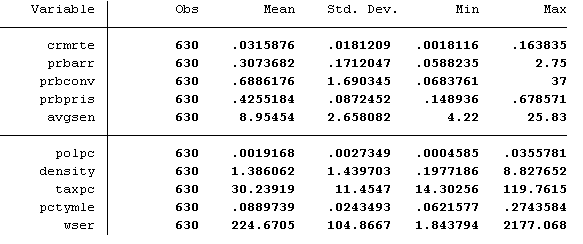
\includegraphics[width=0.7\linewidth]{screenshot002}
	%	\caption{}
	\label{fig:screenshot001}
\end{figure}

However the data is heterogeneous; therefore, scatter plots for the values of interest are plotted on a logarithmic scale: 


\begin{verbatim}
scatter lcrmrte lprbarr
scatter lcrmrte lprbconv
scatter lcrmrte lprbpris
scatter lcrmrte lavgsen
scatter lcrmrte lpolpc
scatter lcrmrte ldensity
scatter lcrmrte lpctymle
scatter lcrmrte county
scatter lcrmrte year
\end{verbatim}


\begin{figure}[htb]
	\begin{minipage}[H]{0.33\linewidth}
		\centering{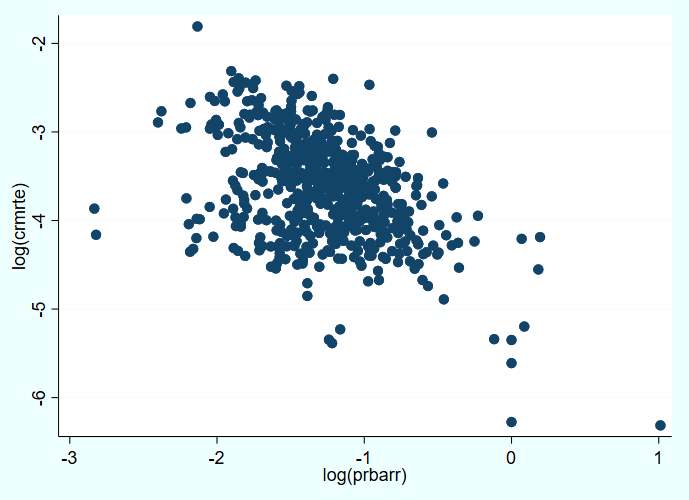
\includegraphics[width=1\linewidth]{screenshot003}}
	\end{minipage}
	\begin{minipage}[H]{0.33\linewidth}
		\centering{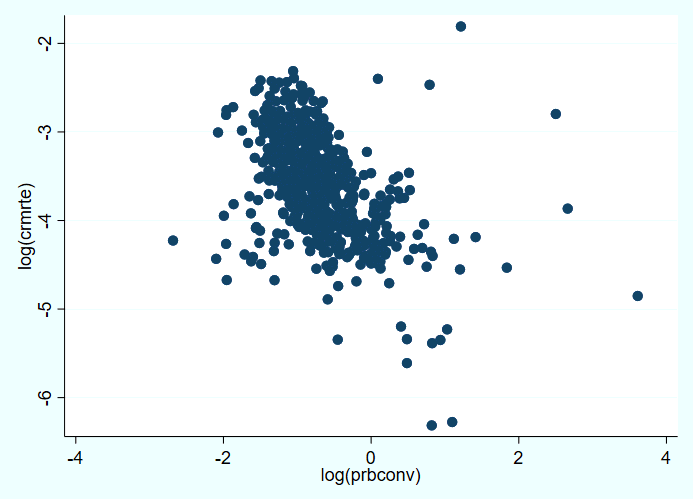
\includegraphics[width=1\linewidth]{screenshot004}}
	\end{minipage}
	\begin{minipage}[H]{0.33\linewidth}
  		\centering{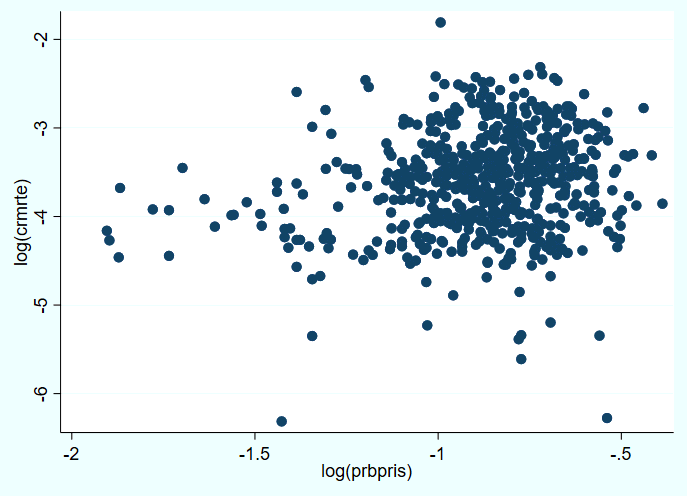
\includegraphics[width=1\linewidth]{screenshot005}}
	\end{minipage}
	\begin{minipage}[H]{0.33\linewidth}
		\centering{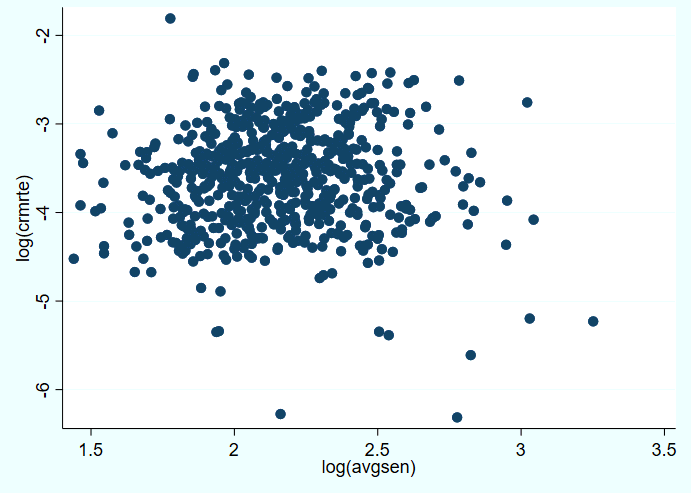
\includegraphics[width=1\linewidth]{screenshot006}}
	\end{minipage}
	\begin{minipage}[H]{0.33\linewidth}
	\centering{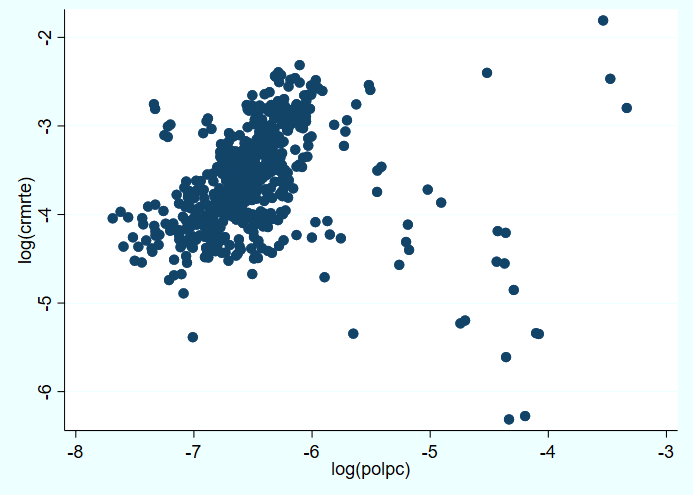
\includegraphics[width=1\linewidth]{screenshot007}}
	\end{minipage}
	\begin{minipage}[H]{0.33\linewidth}
		\centering{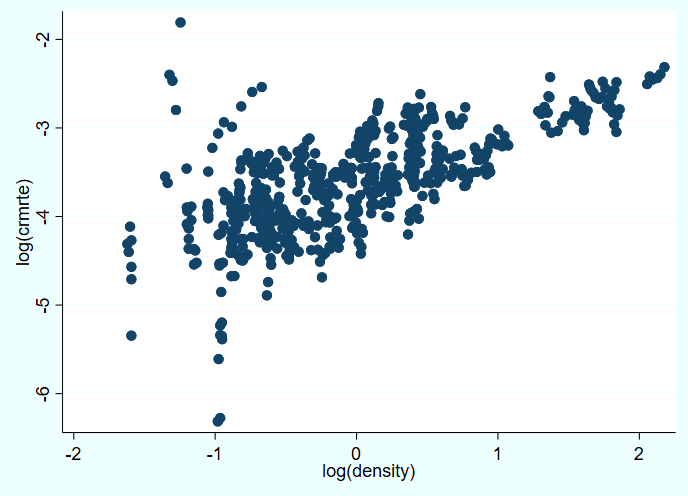
\includegraphics[width=1\linewidth]{screenshot008}}
	\end{minipage}
	\begin{minipage}[H]{0.33\linewidth}
	\centering{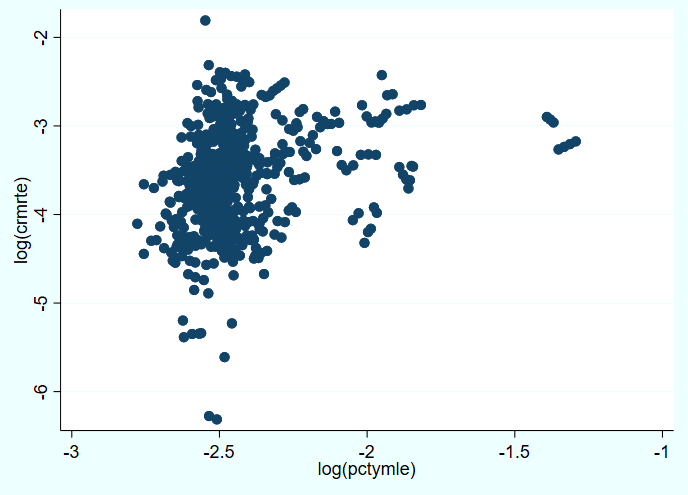
\includegraphics[width=1\linewidth]{screenshot009}}
	\end{minipage}
	\begin{minipage}[H]{0.33\linewidth}
		\centering{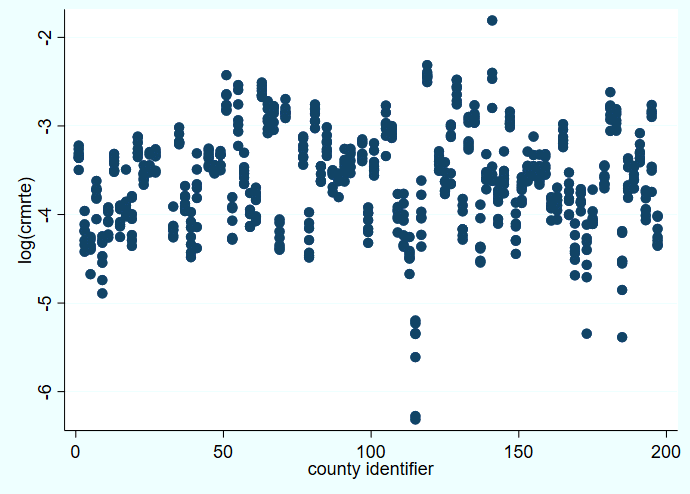
\includegraphics[width=1\linewidth]{screenshot010}}
	\end{minipage}
	\begin{minipage}[H]{0.33\linewidth}
		\centering{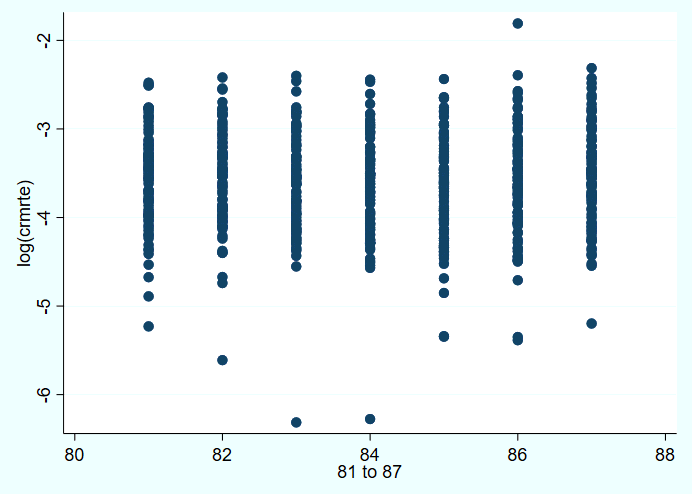
\includegraphics[width=1\linewidth]{screenshot011}}
	\end{minipage}	
\end{figure}

\newpage

\begin{verbatim}
corr lcrmrte lprbarr lprbconv lprbpris lavgsen lpolpc
\end{verbatim}

\begin{figure}[H]
	\centering
	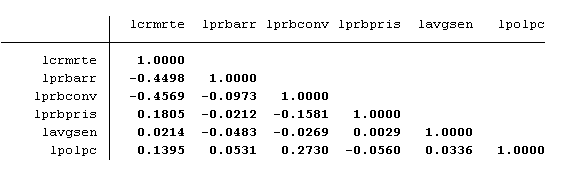
\includegraphics[width=0.7\linewidth]{screenshot001}
%	\caption{}
	\label{fig:screenshot001}
\end{figure}


If all the observation are pooled together no relation can be seen between \texttt{lcrmrte} and \texttt{lprbpris}, \texttt{lcrmrte} and \texttt{lavgsen}, negative relation \texttt{lcrmrte} and \texttt{lprbarr}, \texttt{lcrmrte} and \texttt{lprbconv}. That is if probability to be arrested or to be convicted is low, then crime is higher. However looking on pairplots is not enough, e.g. probability to be convicted might be correlated to police per capita.
Almost no difference can be observed between the \texttt{lcrmrte} grouped by years, however, between the counties the difference can be seen. 


\subsection*{(2)}


\begin{verbatim}
reg lcrmrte lprbarr lprbconv lprbpris lavgsen lpolpc
\end{verbatim}


\begin{figure}[H]
	\centering
	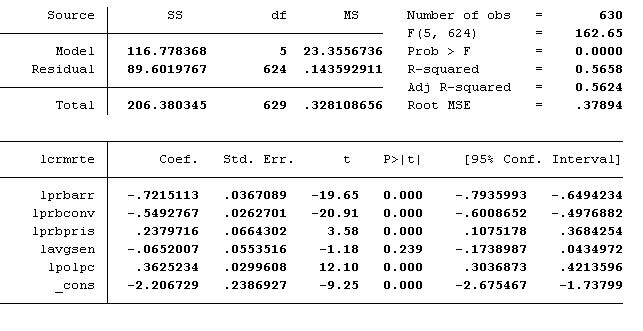
\includegraphics[width=0.7\linewidth]{screenshot012}
	%	\caption{}
	\label{fig:screenshot001}
\end{figure}


If a pooled regression model is chosen to explain  \texttt{lcrmrte}, than it is assumed that there are no unique attributes of individuals within the measurement set, and no universal effects across time. Though, these results can't be realistic, because probably there are some common factor  for  each of the counties.


\subsection*{(3)}

Estimate the same model for each separate cross-section. 

\begin{verbatim}
reg lcrmrte lprbarr lprbconv lprbpris lavgsen lpolpc if year==81
reg lcrmrte lprbarr lprbconv lprbpris lavgsen lpolpc if year==82
reg lcrmrte lprbarr lprbconv lprbpris lavgsen lpolpc if year==83
reg lcrmrte lprbarr lprbconv lprbpris lavgsen lpolpc if year==84
reg lcrmrte lprbarr lprbconv lprbpris lavgsen lpolpc if year==85
reg lcrmrte lprbarr lprbconv lprbpris lavgsen lpolpc if year==86
reg lcrmrte lprbarr lprbconv lprbpris lavgsen lpolpc if year==87
\end{verbatim}


\begin{figure}[htb]
	\begin{minipage}[H]{0.5\linewidth}
		\caption{1981}
		\centering{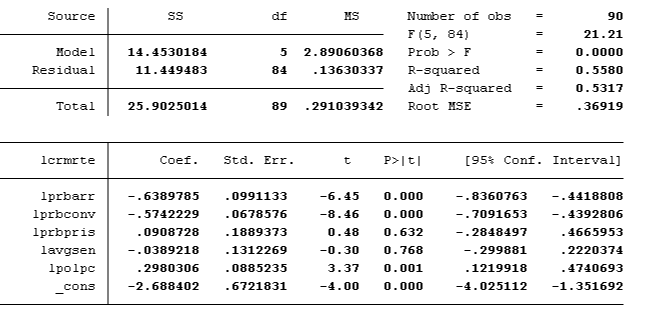
\includegraphics[width=1\linewidth]{screenshot013}}
	\end{minipage}
	\begin{minipage}[H]{0.5\linewidth}
		\caption{1982}
		\centering{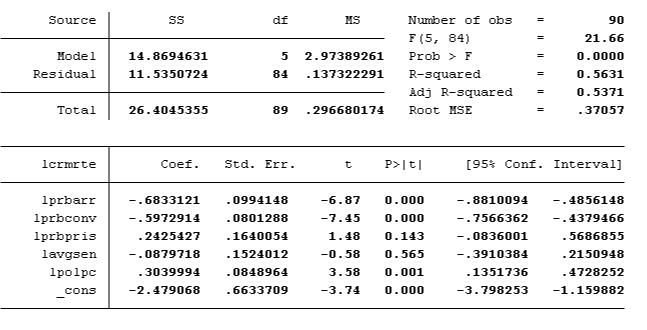
\includegraphics[width=1\linewidth]{screenshot014}}
	\end{minipage}
	\begin{minipage}[H]{0.5\linewidth}
				\caption{1983}
		\centering{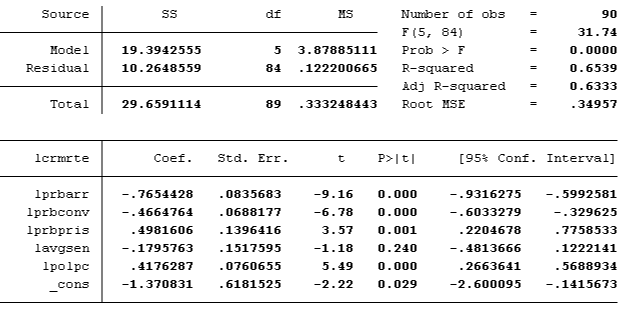
\includegraphics[width=1\linewidth]{screenshot015}}
	\end{minipage}
	\begin{minipage}[H]{0.5\linewidth}
				\caption{1984}
		\centering{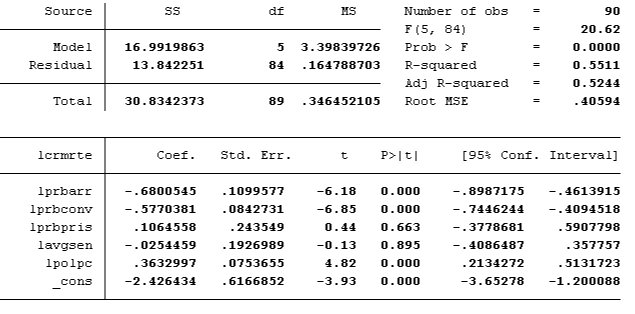
\includegraphics[width=1\linewidth]{screenshot016}}
	\end{minipage}
	\begin{minipage}[H]{0.5\linewidth}
				\caption{1985}
		\centering{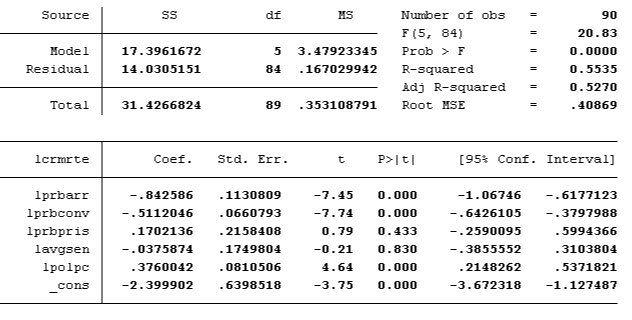
\includegraphics[width=1\linewidth]{screenshot017}}
	\end{minipage}
	\begin{minipage}[H]{0.5\linewidth}
				\caption{1986}
		\centering{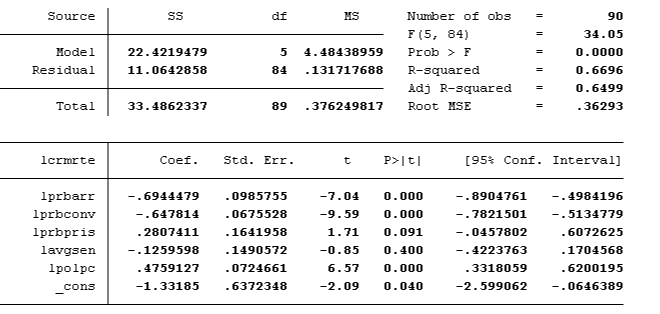
\includegraphics[width=1\linewidth]{screenshot018}}
	\end{minipage}
\end{figure}

\begin{figure}[htb]
\begin{minipage}[H]{0.5\linewidth}
	\caption{1987}
	\centering{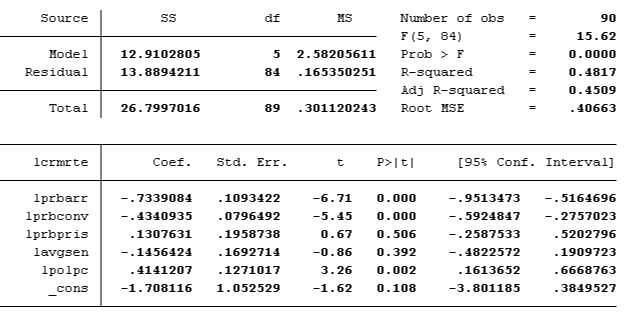
\includegraphics[width=1\linewidth]{screenshot019}}
\end{minipage}
\end{figure}


\newpage

In 1981, 1982, 1984, 1986, 1987 \texttt{lprbpris} is insignificant (on 5\% level), though in pooled regression it has a significant negative effect.  

\subsection*{(4)}

\begin{verbatim}
xtreg lcrmrte lprbarr lprbconv lprbpris lavgsen lpolpc, be
\end{verbatim}

\begin{figure}[H]
	\centering
	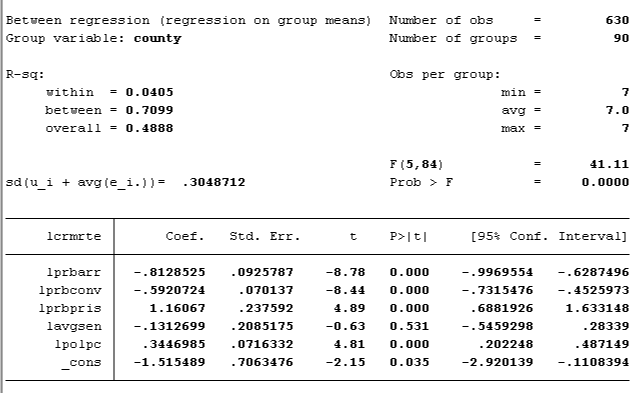
\includegraphics[width=0.7\linewidth]{screenshot020}
	%	\caption{}
	\label{fig:screenshot001}
\end{figure}


In “between” regression in comparison to pooled  \texttt{lprbpris} has much stronger effect, and in comparison to most of the regressions  on cross-section  data this effect is significant. Other significant coefficient estimates are roughly the same.

\newpage

\subsection*{(5)}


\begin{verbatim}
xtreg lcrmrte lprbarr lprbconv lprbpris lavgsen lpolpc, fe
\end{verbatim}



\begin{figure}[H]
	\centering
	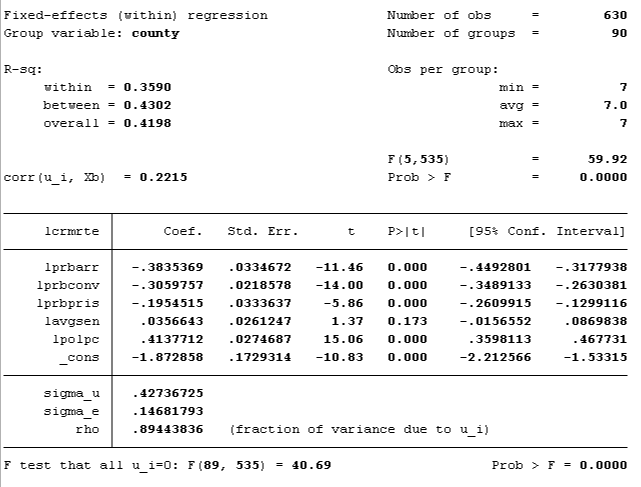
\includegraphics[width=0.7\linewidth]{screenshot021}
	%	\caption{}
	\label{fig:screenshot001}
\end{figure}

In fixed effects model in comparison to between-estimates   the estimates of \texttt{lprbarr} and \texttt{lprbconv} are still significant, but are almost twice smaller by absolute value.  The estimate of \texttt{lprbpris} is significant, but in comparison to between-estimates it becomes negative.
Cornwell and Trumbull concluded that cross-section estimates do not account for an individual effect, therefore, are misleading.



\subsection*{(6)}
\begin{figure}[H]
	\centering
	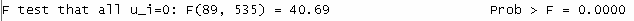
\includegraphics[width=0.7\linewidth]{screenshot038}
	%	\caption{}
	\label{fig:screenshot001}
\end{figure}



To test the fixed effects model against the pooled regression model, F-test is used. The test is significant, i.e., hypothesis that all counties' effects are equal to 0 is rejected, therefore, the fixed effects model is preferred over pooled regression.



\newpage

\subsection*{(7)}

\begin{verbatim}
xtreg lcrmrte lprbarr lprbconv lprbpris lavgsen lpolpc, fe
predict uu, u
local list "lcrmrte lprbarr lprbconv lprbpris lavgsen lpolpc"

foreach xx of local list {
	display "`xx'"
	xtreg `xx', fe
	predict mm, xb
	predict u1, u
	gen tm_`xx' = u1+mm
	drop u1 mm
}

reg uu west central urban pctmin80 tm_lprbarr tm_lprbconv tm_lprbpris 
tm_lavgsen tm_lpol
\end{verbatim}

\begin{figure}[H]
	\centering
	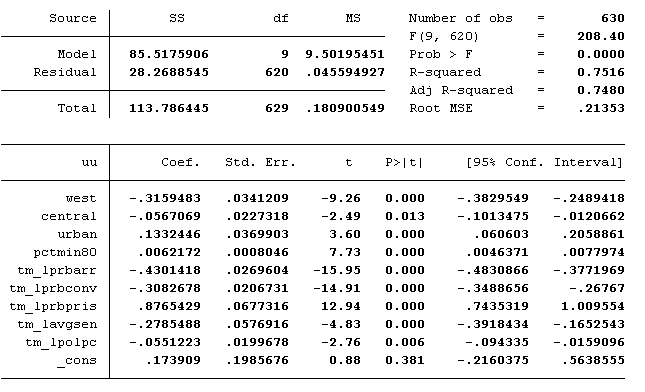
\includegraphics[width=0.7\linewidth]{screenshot028}
	%	\caption{}
	\label{fig:screenshot001}
\end{figure}

In western and central North Carolina crime rate is lower, in urban counties and counties with higher minority percentage -- higher.

\newpage

\subsection*{(8)}

\begin{verbatim}
xtreg lcrmrte lprbarr lprbconv lprbpris lavgsen lpolpc d8*, fe
test d82 d83 d84 d85 d86 d87
\end{verbatim}

%\begin{figure}[H]
%	\centering
%	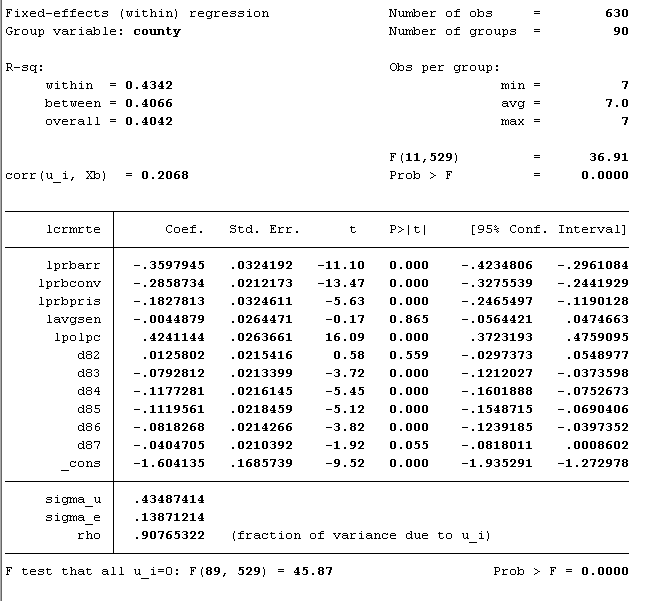
\includegraphics[width=0.7\linewidth]{screenshot029}
%	%	\caption{}
%	\label{fig:screenshot001}
%\end{figure}


\begin{figure}[H]
	\centering
	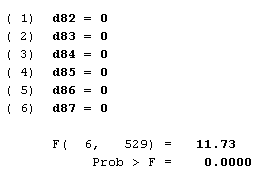
\includegraphics[width=0.35\linewidth]{screenshot030}
	%	\caption{}
	\label{fig:screenshot001}
\end{figure}

By F-test we conclude that dummy variables are significant, therefore, it can be useful to account for time dummies. 


\subsection*{(9)}


\begin{verbatim}
xtreg lcrmrte lprbarr lprbconv lprbpris lavgsen lpolpc d8* 
ldensity lwcon lwtuc lwtrd lwfir lwser lwmfg lwfed lwsta lwloc 
lpctymle ltaxpc lmix, fe
\end{verbatim}



\begin{figure}[H]
	\centering
	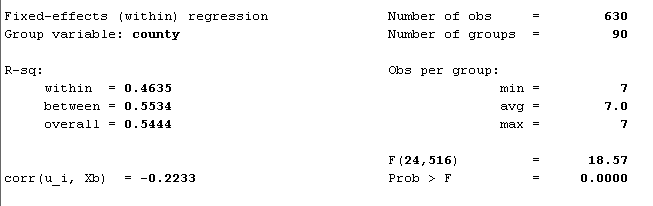
\includegraphics[width=0.9\linewidth]{screenshot031}
	%	\caption{}
	\label{fig:screenshot001}
\end{figure}




\begin{figure}[H]
	\centering
	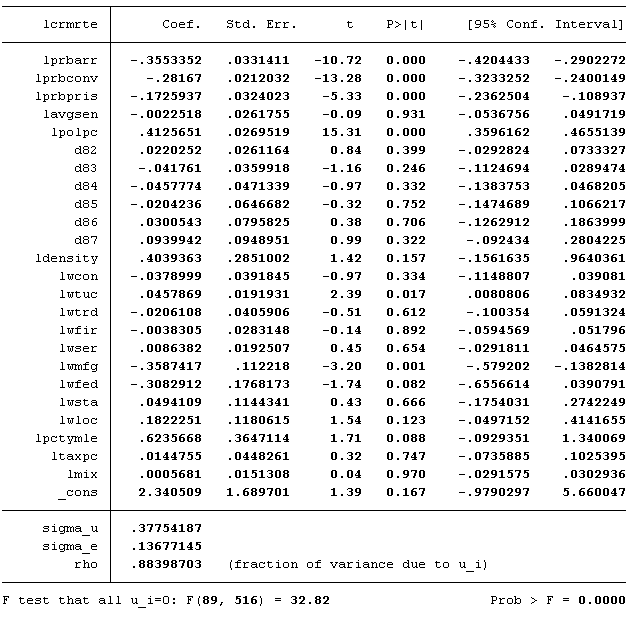
\includegraphics[width=0.7\linewidth]{screenshot032}
	%	\caption{}
	\label{fig:screenshot001}
\end{figure}


With all the time-varying regressors \texttt{lprbpris} is again significant and negative.

Coefficient of \texttt{lpctymle} is positive and significant, therefore, if crime rate is positively dependent on percentage of young male, the government should  work on programs to lower unemployment rate for this group, provide them with education programs, etc. 

Higher wages for tranport, utility and communal servives correspond to higher   crime rates (this may be caused by the fact that this type of job doen't require a university degree but  specific skills are needed, so if wages in this sector are higher the competition is also higher; therefore, some groups, especially the ones in need,  can't get the job and might commit crime), higher wages for manufacturing lowers crime rate (this job is quite hard and in most cases not payed as well, so in counties where workers are underpayed more crimes are commited).

\newpage 

\subsection*{(10)}

\begin{verbatim}
xtreg lcrmrte lprbarr lprbconv lprbpris lavgsen lpolpc, re
\end{verbatim}


\begin{figure}[H]
	\centering
	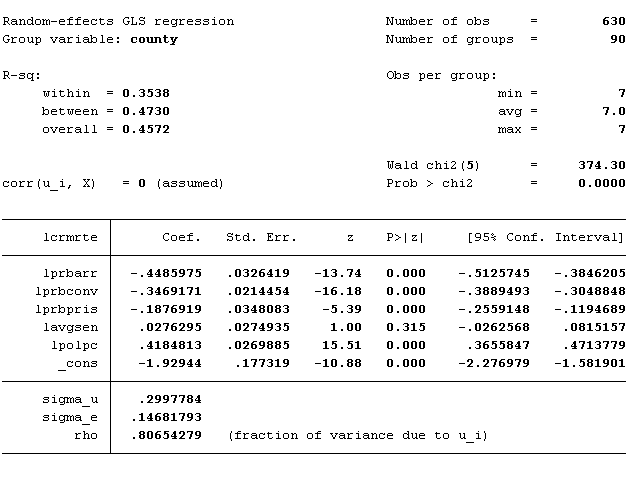
\includegraphics[width=0.7\linewidth]{screenshot033}
	%	\caption{}
	\label{fig:screenshot001}
\end{figure}



Random effects model assuming that the unique, time constant attributes of individuals that are not correlated with the individual regressors. The same regressors have significant estimates of their coefficients, with the same signs as in FE-model.  


\subsection*{(11)}

\begin{verbatim}
xttest0
\end{verbatim}

\begin{figure}[H]
	\centering
	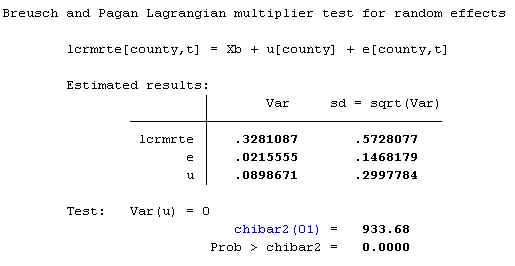
\includegraphics[width=0.7\linewidth]{screenshot034}
	%	\caption{}
	\label{fig:screenshot001}
\end{figure}

To test the random effects model in comparison to pooled
regression model Breusch-Pagan LM-test is used, where the null is is that the variance of the unobserved fixed effects is zero. The null is rejected therefore RE should be prefered over pooled regression.




\begin{verbatim}
xtreg lcrmrte lprbarr lprbconv lprbpris lavgsen lpolpc, re
est store RE
xtreg lcrmrte lprbarr lprbconv lprbpris lavgsen lpolpc, fe
est store FE
hausman FE RE, sigmamore
\end{verbatim}

\begin{figure}[H]
	\centering
	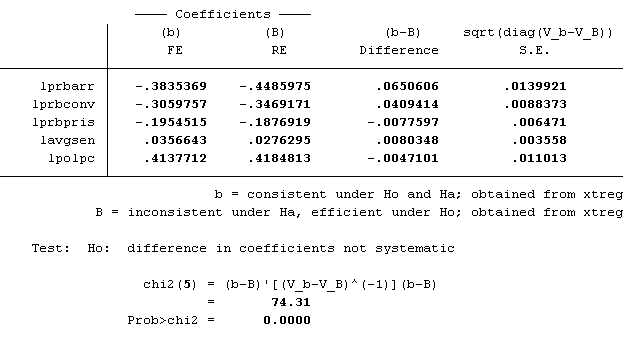
\includegraphics[width=0.7\linewidth]{screenshot037}
	%	\caption{}
	\label{fig:screenshot001}
\end{figure}


Test the random effects model in comparison to  fixed effects model Hausman test is used.
The unique attributes of individuals may or may not be correlated with the individual dependent variables. Under null hypothesis individual effects and the regressors are uncorrelated. In this case it is rejected; therefore, RE-estimates are inconsistent and FE is prefered over RE.  


\end{document}
